\begin{refsection}

	\chapter{Disseny i programació de xarxes neuronals}
	\label{chap:pract}

	La finalitat del treball és l'aplicació dels conceptes de xarxes neuronals. Es provaran xarxes neuronals simples amb diferents funcions d'activació per veure el seu comportament i la seva precisió. Com a base del projecte, s'ha utilitzat la base de dades \textbf{MNIST}, \cref{fig:mnist}, un conjunt d'imatges de dígits escrits a mà que són emprats per a l'entrenament de sistemes de classificació automàtica d'imatges. És l'evolució de la base de dades NIST. MNIST consta d'un conjunt de 70000 dígits manuscrits: 60000 imatges per entrenar la xarxa neuronal i 10000 imatges per mesurar la seva eficiència.\supercite{MNIST}
	
	\begin{figure}[h]
		\centering
		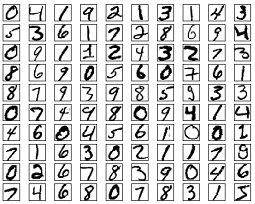
\includegraphics[width=8cm]{mnist}
		\caption{Base de dades MNIST}
		\label{fig:mnist}
	\end{figure}

	Pel que fa a les tecnologies i \textit{frameworks} d'aprenentatge profund, hi ha diverses eleccions a considerar: \textbf{TensorFlow}, \textbf{Keras}, \textbf{PyTorch}:
	
	\begin{itemize}
		\item \textbf{TensorFlow} és una biblioteca de programari de codi obert per a l'aprenentatge profund i automàtic desenvolupada per l'equip Google Brain per satisfer les seves necessitats de crear i entrenar xarxes neuronals per detectar i desxifrar patrons i correlacions. S'utilitza tant per a la investigació com per a la producció a Google i està sota la llicència Apache 2.0.\supercite{TensorFlow}
		
		En aquest projecte s'utilitzarà TensorFlow per la seva capacitat per realitzar un bon rendiment a càlculs de nivell baix i alt. També, a causa de la naturalesa de processament d'imatges del projecte i la seva capacitat d'integració fàcil amb altres biblioteques Python com NumPy\supercite{NumPy} o PIL.\supercite{Pillow}
		
		\item \textbf{Keras} és una biblioteca de xarxes neuronals de codi obert escrita en llenguatge Python. Keras es pot executar damunt de TensorFlow, Microsoft Cognitive Toolkit (CNTK) o Theano. Va ser desenvolupat per l'experimentació en xarxes neuronals. Els seus advantages són la facilitat d'ús, modularitat i extensibilitat.\supercite{Keras}
		
		\item \textbf{PyTorch} és una biblioteca de programari de codi obert per a l'aprenentatge automàtic, basada en la biblioteca Torch i escrita en Python, C++ i CUDA. És desenvolupada principalment pel grup de recerca d'intel·ligència artificial de Facebook.\supercite{PyTorch}
		
		
	\end{itemize}

	Com ja s'ha indicat anteriorment, un dels objectius del treball és aconseguir un valor de precisió el més proper al $100\%$ possible. Això s'aconsegueix mitjançant la configuració ideal de les variables com ara els pesos o els biaixos.
	
	L'activitat consisteix en programar una xarxa neuronal en la qual la sortida generada sigui el valor del número que la xarxa ha obtingut com a entrada però en format d’imatge. Ès a dir, la xarxa ha d'endevinar quin es el número escrit a mà. Com més encerti, obtindrà un valor de precisió o més
	elevat.
	
	Per aconseguir aquests valors, es diferencien dues fases de modelització
	
	\begin{itemize}
		\item \textit{Fase d’entrenament}. En aquesta fase s’utilitza una part
		del conjunt de dades (MNIST en aquest cas) per determinar els pesos que defineixen el model de la xarxa neuronal. Aquests pesos es calculen de manera iterativa, amb l'objectiu de minimitzar l'error obtingut entre la sortida resultant de la xarxa i el valor de sortida desitjat.
		
		Un altre concepte que s'utilitza en l'entrenament consisteix en la \textit{retropropagació} o \textit{backpropagation}.\supercite{backprop} És un metode de càlcul de pesos que s'utilitza en algoritmes d'aprenentatge i que ofereix molt bons resultats gràcies al reajustament dels pesos de les neurones en direcció contrària després d’haver recorregut la xarxa des del principi fins al final.
		
		Durant aquesta fase, el model pot patir un \textit{sobreentrenament}, de manera que s’ajusta massa a les particularitats del patró d'entrenament. En aquest cas es perdria l'habilitat de generar el seu aprenentatge en nous casos amb altres dades.
		
		\item \textit{Fase de prova}. Per evitar el problema del sobreentrenament, s'utilitza un segon
		grup de dades diferents de les d'entrenament per permetre controlar el procés d'aprenentatge.
		
		Aquest grup de dades s'utilitza per veure com reacciona el model davant dades que no ha analitzat anteriorment i es pot saber quin és el seu grau de precisió i el seu grau d'error.

	\end{itemize}

	El primer pas en el desenvolupament del projecte consisteix en crear una xarxa neuronal bàsica d'una sola capa. Aquesta vindria representada per 784 unitats d'entrada, que corresponen al nombre de píxels que conté la imatge del model de dades (24x24 píxels), i 10 sortides, que representen els deu possibles dígits $[0 - 9]$ de la imatge d'entrada.
	
	\begin{figure}[h]
		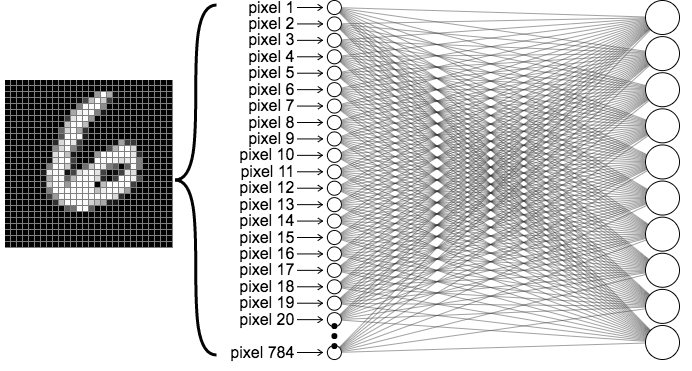
\includegraphics[width=\textwidth]{mnist1layer}
		\caption{Xarxa bàsica per MNIST\protect\supercite{Ml4a}}
	\end{figure}

	\section{Entorn}
	
	Primer de tot, cal destacar l’entorn dels experiments, tant el \textit{hardware} com el \textit{software}:
	
	\begin{itemize}
		\item CPU: Intel Core i7-8750H
		\item GPU: NVIDIA GeForce GTX 1060
		\item RAM: 16 GB DDR4
		\item OS: Windows 10
		\item \textbf{Python}. És un dels llenguatges de programació més utilitzats per experiments amb IA. És un llenguatge multiplataforma, orientat a objectes i fàcil d'aprendre gràcies a la seva sintaxi. Ha estat escollit per la gran quantitat de biblioteques, tipus de dades i funcions
		incorporades en el mateix llenguatge, que ajuden a realitzar moltes tasques sense necessitat de programar-les de zero.\supercite{Python}
		\item \textbf{TensorFlow}. Un dels \textit{frameworks} més utilitzats per realitzar la gestió de xarxes neuronals.\supercite{TDS10}
		\item \textbf{Keras}. S'executa per damunt de TensorFlow. Biblioteca de Python que proporciona, d'una manera simple i eficient, la creació de models de xarxes neuronals.\supercite{Keras,TDS10}
		\item \textbf{Anaconda}. És una distribució de codi obert dels llenguatges de programació Python.\supercite{Anaconda}
		\item \textbf{Jupyter Notebook}. És un entorn computacional interactiu basat en la web per crear documents de quaderns Jupyter (\textit{notebooks}) en llenguatge Python.\supercite{Jupyter}
	\end{itemize}

	\section{Xarxa neuronal}
	
	El primer pas realitzat consisteix en carregar el model de dades MNIST explicat anteriorment per a poder tractar-lo. Keras ja incorpora el conjunt de dades MNIST i només cal importar-lo i guardar-lo en les variables d'entrenament i test. Un cop fet, només cal preprocessar correctament les dades carregades d'aquest conjunt, com es mostra en el \cref{lst:first}.
	
	En aquest punt, tenim 60000 mostres de dígits del 0 al 9, escrits a mà, en una variable llesta per ser tractada per la xarxa que es crea a continuació.
	
	\begin{listing}[H]
		\begin{pythoncode}
# TensorFlow
import tensorflow as tf
# Model Sequential, pila lineal de capes de xarxes neuronals
from tensorflow.keras.models import Sequential
# Capes bàsiques de Keras
from tensorflow.keras.layers import Dense, Dropout, Activation, Flatten
# Utilities
from tensorflow.python.keras.utils import to_categorical

# Importar el conjunt de dades MNIST i guardar-lo en variables
from tensorflow.python.keras.datasets import mnist
(X_train, y_train), (X_test, y_test) = mnist.load_data()

# Preprocessar les dades
X_train = X_train.reshape(X_train.shape[0], 784)
X_test = X_test.reshape(X_test.shape[0], 784)
X_train = X_train.astype('float32')
X_test = X_test.astype('float32')
# Normalitzar els valors a l'interval [0, 1]
X_train /= 255
X_test /= 255
# Obtenir 10 classes per als dígits 0-9
Y_train = to_categorical(y_train, 10)
Y_test = to_categorical(y_test, 10)
\end{pythoncode}
		\caption{Importar MNIST i preprocessar les dades}
		\label{lst:first}
	\end{listing}

	El següent pas consisteix en la creació del model de la xarxa (\cref{lst:model}). Primerament, s’ha creat una xarxa amb estructura bàsica on les entrades es connecten directament amb les 10 neurones de sortida (una per cada dígit del 0 al 9, \cref{fig:mnistann1}). Seguidament es fa la compilació i lentrenament de la xarxa.

	\begin{listing}[H]
		\begin{pythoncode}
# Model
model = Sequential()
model.add(Dense(10, activation='sigmoid', input_shape=(784,)))

# Compilació del model
model.compile(loss='binary_crossentropy',
			  optimizer='adam', metrics=['accuracy'])

# Entrenament
hist = model.fit(X_train, Y_train,
				validation_data=(X_test, Y_test),
				epochs=20, verbose=1)
\end{pythoncode}
		\caption{Model de xarxa neuronal}
		\label{lst:model}
	\end{listing}
	
	\begin{figure}[H]
		\centering
		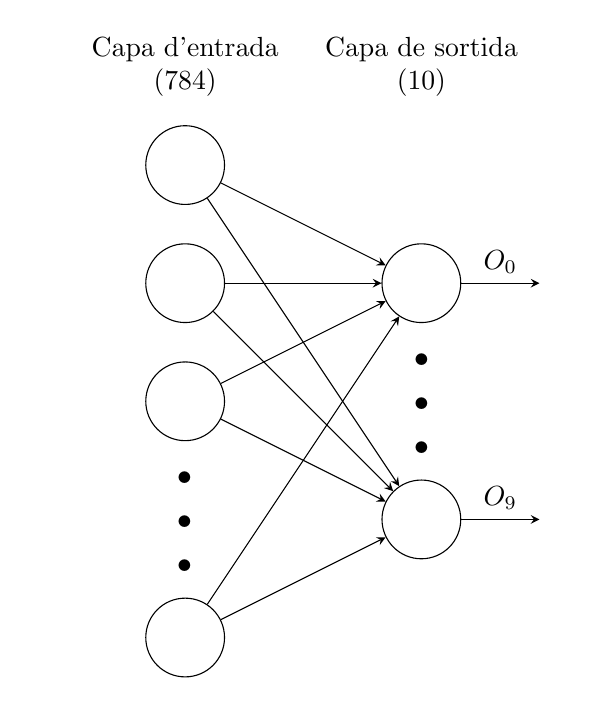
\begin{tikzpicture}[x=1.5cm, y=1.5cm, >=stealth,
		every neuron/.style={
			circle,
			draw,
			minimum size=1cm
		},
		neuron missing/.style={
			draw=none, 
			scale=4,
			text height=0.333cm,
			execute at begin node=\color{black}$\vdots$
		},
		]
		
		\foreach \m/\l [count=\y] in {1,2,3,missing,4}
		\node [every neuron/.try, neuron \m/.try] (input-\m) at (0,2.5-\y) {};
		
		\foreach \m [count=\y] in {1,missing,2}
		\node [every neuron/.try, neuron \m/.try ] (output-\m) at (2,1.5-\y) {};
		
		\foreach \l [count=\i] in {0,9}
		\draw [->] (output-\i) -- ++(1,0)
		node [above, midway] {$O_\l$};
		
		\foreach \i in {1,...,4}
		\foreach \j in {1,...,2}
		\draw [->] (input-\i) -- (output-\j);
		
		\node [align=center, above] at (0,2) {Capa d'entrada\\(784)};
		\node [align=center, above] at (2,2) {Capa de sortida\\(10)};
		\end{tikzpicture}
		\caption{Xarxa neuronal}
		\label{fig:mnistann1}
	\end{figure}

	El model creat representa un model seqüencial amb 784 entrades per una capa de 10 sortides i una funció d'activació sigmoide presentada anteriorment.
	
	Fins ara, hem aconseguit construir una xarxa neuronal capaç d'identificar dígits del 0 al 9 amb un percentatge d'encert prou alt. La \cref{fig:acc1,fig:loss1} mostra els resultats obtinguts mitjançant aquesta xarxa. Es poden observar dos gràfics que representen els valors \textit{accuracy} (precisió) i \textit{loss} (error) respecte les \textit{epochs}, és a dir, el percentatge d'encert i el valor d'error respecte a cada iteració del model.
	
	\begin{figure}[H]
		\centering
		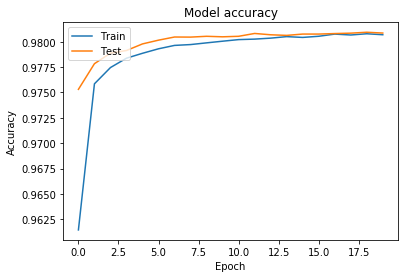
\includegraphics[width=.75\textwidth]{acc1}
		\captionof{figure}{Precisió de la xarxa}
		\label{fig:acc1}
	\end{figure}

	\begin{figure}[H]
		\centering
		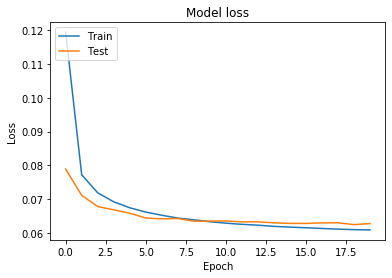
\includegraphics[width=0.75\textwidth]{loss1}
		\captionof{figure}{Error de la xarxa}
		\label{fig:loss1}
	\end{figure}

	Les modificacions posteriors de la xarxa neuronal amb la finalitat d'aconseguir més eficiència i l'applicació amb GUI (\cref{fig:app1,fig:app2}) es poden trobar a \cite{mygithub}.
	
	\begin{figure}[H]
		\centering
		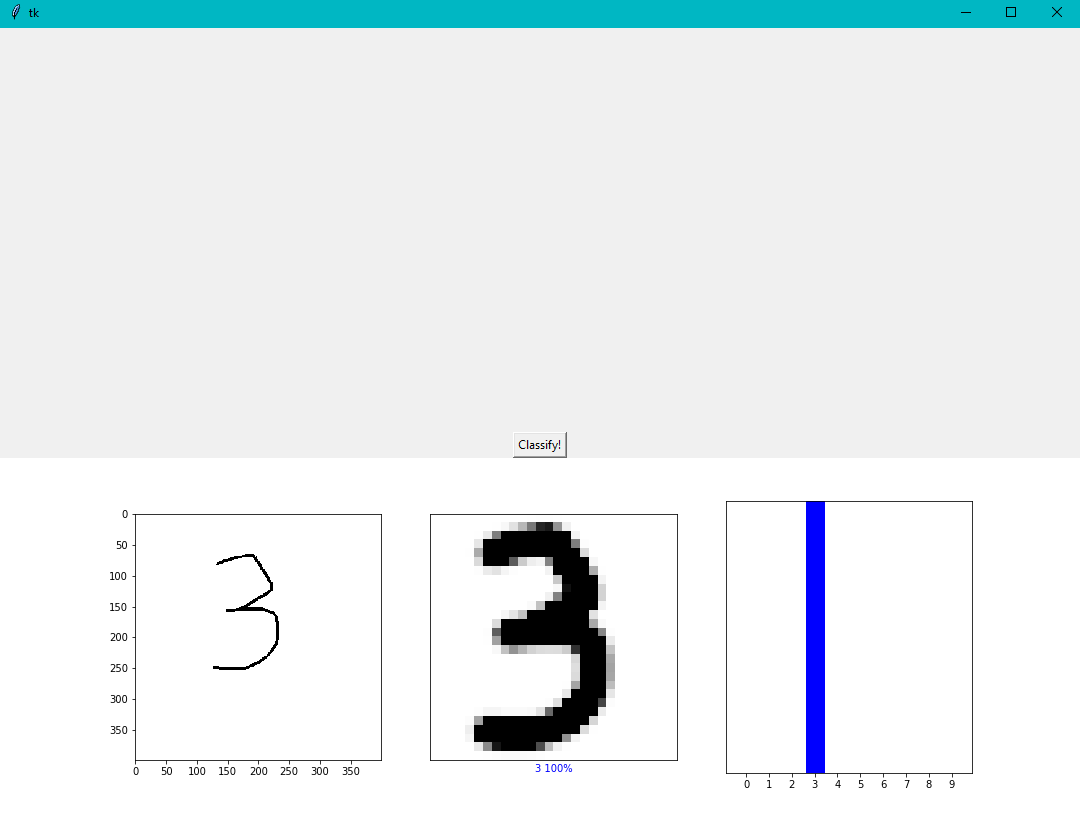
\includegraphics[width=.75\textwidth]{app3}
		\captionof{figure}{Applicació GUI}
		\label{fig:app1}
	\end{figure}

	\begin{figure}[H]
		\centering
		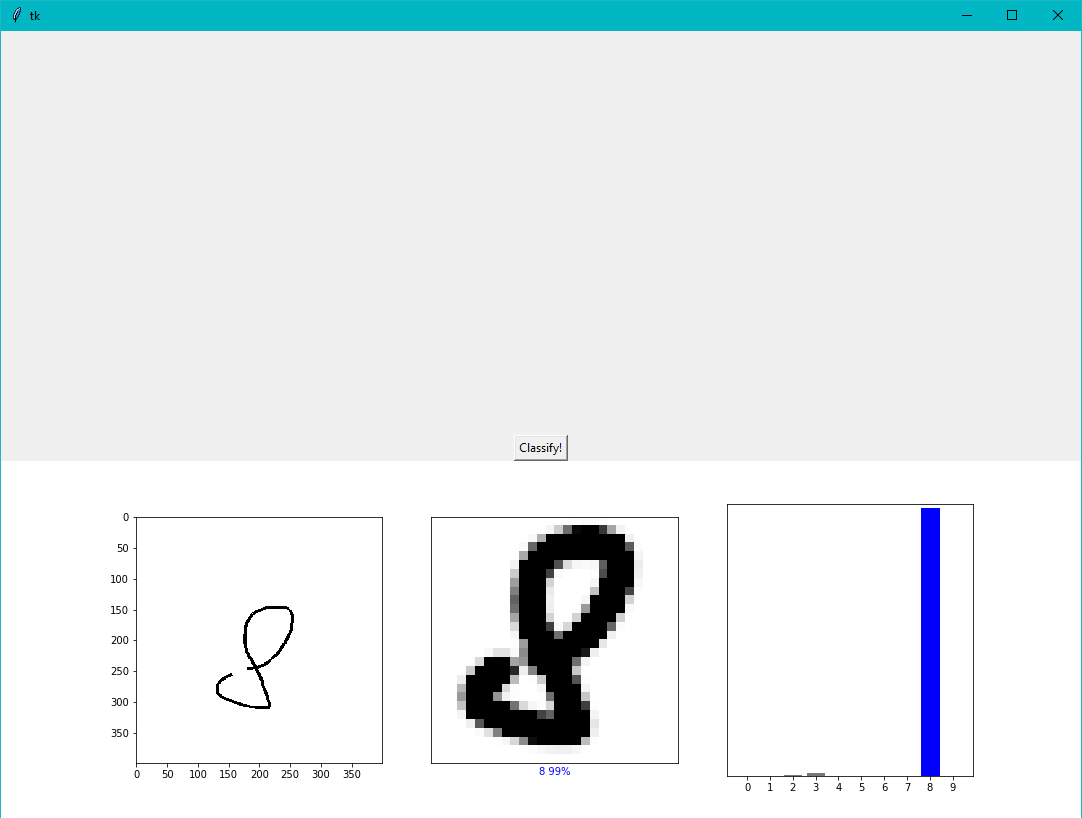
\includegraphics[width=.75\textwidth]{app8}
		\captionof{figure}{Applicació GUI}
		\label{fig:app2}
	\end{figure}

	\addtocontents{toc}{\vspace{1em}}
	\printbibliography[heading=subbibintoc]

\end{refsection}
